\chapter{\begin{center}
    \textcolor{purple}{Présentation générale du projet}
\end{center}}
\section*{\textcolor{cyan}{Introduction}}
L’étude de projet est une démarche stratégique visant à organiser le bon déroulement d’un projet et d’assurer la conduite de toutes les phases qui le constituent.\par
Une étude complète et efficace conduit généralement à la réussite d’un projet. Cette étude fera donc l’objet de notre premier chapitre qui sera consacré à la présentation de l’organisme d’accueil, et la présentation du projet.\par
\section{\textcolor{cyan}{Présentation de l’organisme d’accueil :}}
Djagora Fablab est le 6éme fablab issu d'un partenariat entre la \textbf{Fondation Orange} et La \textbf{Fondation Djagora}.\par
Situé à la Technopole de Sfax, au village de l'entrepreneuriat, Djagora Fablab intervient dans la chaine de valeur de création de start-up et de l'innovation, coté formation et prototypage.\par
Djagora Fablab est un ouvert au public mettant à la disposition de ses utilisateurs les ressources techniques, technologiques et humaines nécessaires à la conception, l’optimisation, la réparation de toute sorte d’objets.\par
Le Fablab dispose d'une large gamme d'outils de fabrication, notamment une découpeuse laser, une fraiseuse numérique, une imprimantes 3D, un Workstation Pro, etc...
\par
\begin{center}
    
\includegraphics[width=5cm]{images/djagora2.png}
    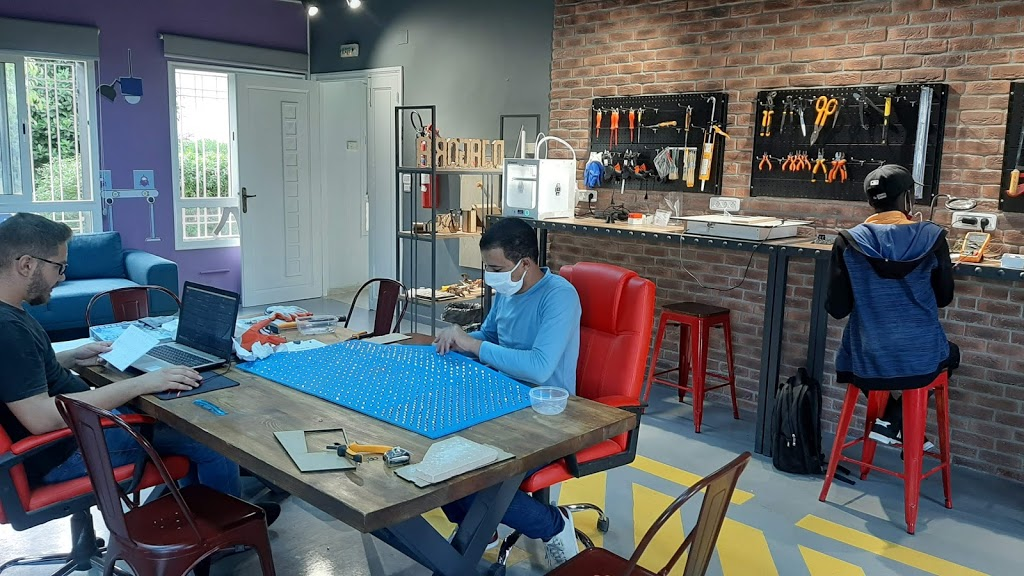
\includegraphics[width=10cm]{images/djagoraImage.png}
    \caption{\textbf{Djagora}}
    \label{fig:my_label}\\
\end{center}
\textbf{\textcolor{cyan}{Djagora Academy:}}\par
Djagora Academy est un programme a pour but d’accélérer l’employabilité des jeunes de l’enseignement supérieur. Il s’adresse essentiellement aux étudiants jeunes diplômés ou en fin de cycle Licence, Master ou Ecole d’Ingénieur.\par
Le programme Djagora Academy repose sur 3 piliers essentiels:\par
\begin{itemize}
    \item Le savoir-être
    \item Le savoir-faire
    \item La réalisation de prototype
\end{itemize}\par
\begin{center}
    
\includegraphics[width=5cm]{images/djagoraAcademy.png}\\
\end{center}
Sur une durée de 5 à 6 mois les étudiants vont developper l’ensemble des compétences recherchées par les employeurs en mettant en pratique toutes les connaissances théoriques apprises au cours de leur cursus académique.\par
Chaque étudiant aura l’opportunité de mettre en pratique ses compétences en “critical thinking” par la conception et la formalisation écrite d’un problème réel en projet, la mobilisation de l’ensemble des parties prenantes grâce à la formation Leadership, la communication au tour du projet grâce à la formation en Digital Marketing, le management de projet grâce à l’outil SCRUM Agile, le travail en équipe grâce au Leadership immersion camp lors de la semaine d’intégration. Enfin, l’approche entrepreneurial grâce a la participation aux compétitions pour startup et salons. Les étudiants ayant participés au programme bénéficient de certifications professionnelles telles que le Six Sigma, le Digital Marketing et SCRUM Agile reconnues au niveau internationale. Nos étudiants se démarquent par le fait d’avoir eu l’opportunité d’appliquer l’ensemble des outils relatifs à ces certifications professionnelles dans des projets réels et ce dans un environnement qui encourage la prise de risque. Le rôle des mentors reste clé dans la réalisation de ce programme.\par
\section{\textcolor{cyan}{Présentation du projet:}}
\subsection{Problème :}
D’un côté, des plateformes de contenus de plus en plus complexes. De l’autre, des publics difficiles à capter, sur-sollicités…\par
Dans ce contexte, la vidéo online est l’un des rares médias qui rende l’information intelligible, attractive, qui valorise les individus, encourage la participation et le dialogue.\par
La WebTV nous est apparue comme étant la scénarisation la plus efficace des contenus vidéo.\par
\subsection{Technologies utilisées:}
\textbf{Node.js} est une plateforme logicielle libre en JavaScript, orientée vers les applications réseau évènementielles hautement concurrentes qui doivent pouvoir monter en charge.
\textbf{Express.js} est un framework pour construire des applications web basées sur Node.js. C'est de fait le framework standard pour le développement de serveur en Node.js.\par
La figure 2 représente les logos de Node.js et Express.js.\par
\begin{center}
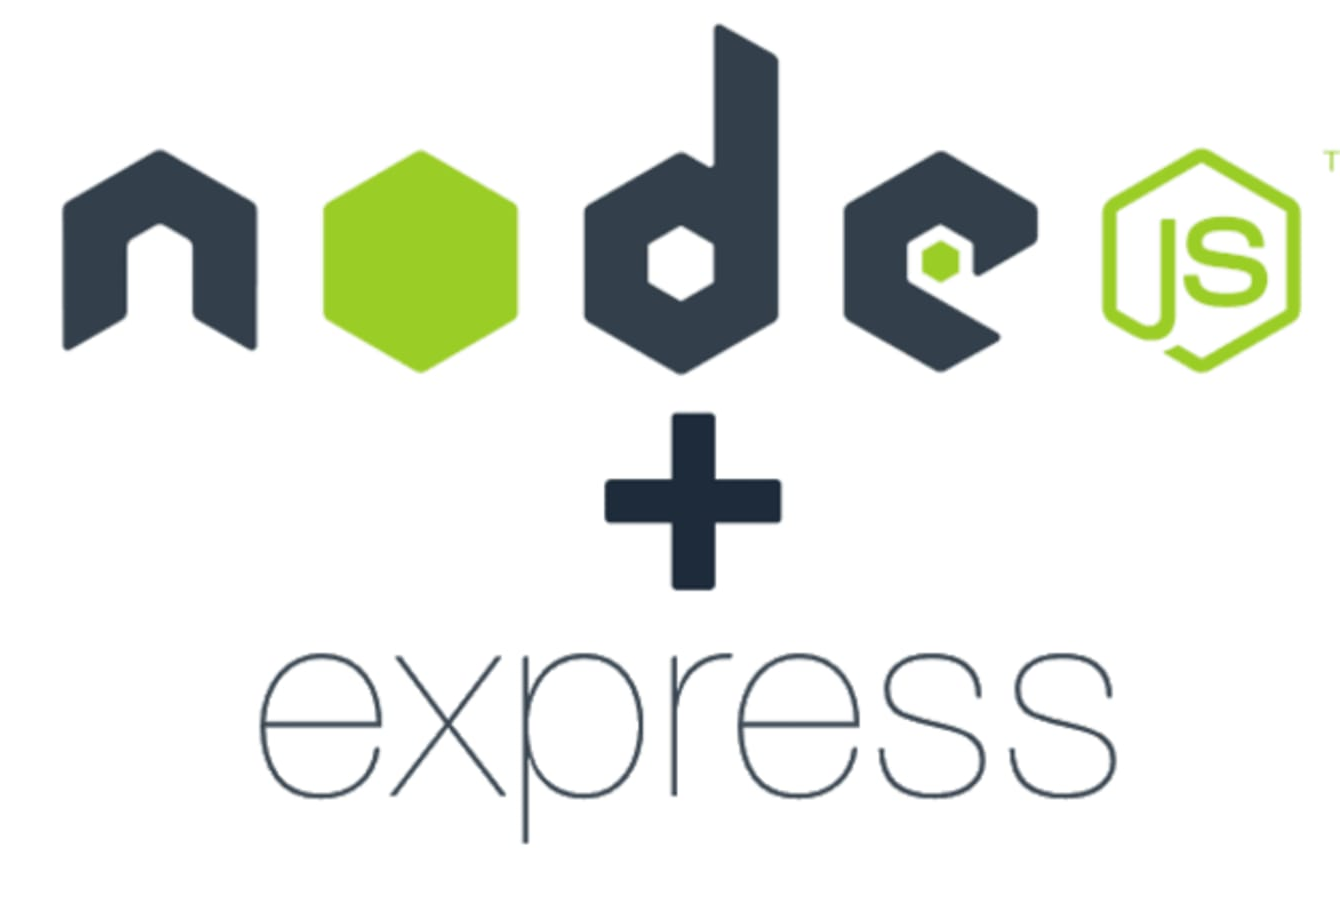
\includegraphics[width=5cm]{images/nodeexpress.png}
     \caption{logos de Node.js et Express.js}
     \label{fig:my_label}\\
\end{center}
\subsubsection{\textbf{Node.js Express VS PHP:}}
Les frameworks PHP modernes améliorent beaucoup leur qualité de code, mais ces frameworks sont encore très en retard par rapport à Node.js en termes de fonctionnalités et de productivité.\par
 PHP est verbeux, peu flexible, et difficile à débogguer. Parce qu'il est conçu pour sa facilité d'utilisation plutôt que pour la qualité du code, il est trop facile d'écrire du code insécure (présentant des failles de sécurité) ou du code spaghetti.\par
\subsubsection{\textbf{Architecture MVC}}[hb]
MVC(Figure2) est un patron de conception(Design Pattern) très répandu pour réaliser la structure des sites web. Ce patron de conception est une solution éprouvée et reconnue permettant de séparer l’affichage des informations, les actions de l’utilisateur et l’accès aux données.En effet, il permet de faciliter le dialogue l’utilisateur et le serveur d’application et d’augmenter les performances de l’application.\par
 Ce modèle comporte trois types de module:\par
 \begin{itemize}
     \item Un modèle (Model) faite grace NodeJS Express.
     \item Une vue (View) contient les pages (CSS+HTML+ JS).
     \item Un contrôleur (Controller) contient les scripts JS qui permet la logique concernant les actions effectuées par l'utilisateur.
 \end{itemize}
 \begin{figure}[hb]
     \centering
     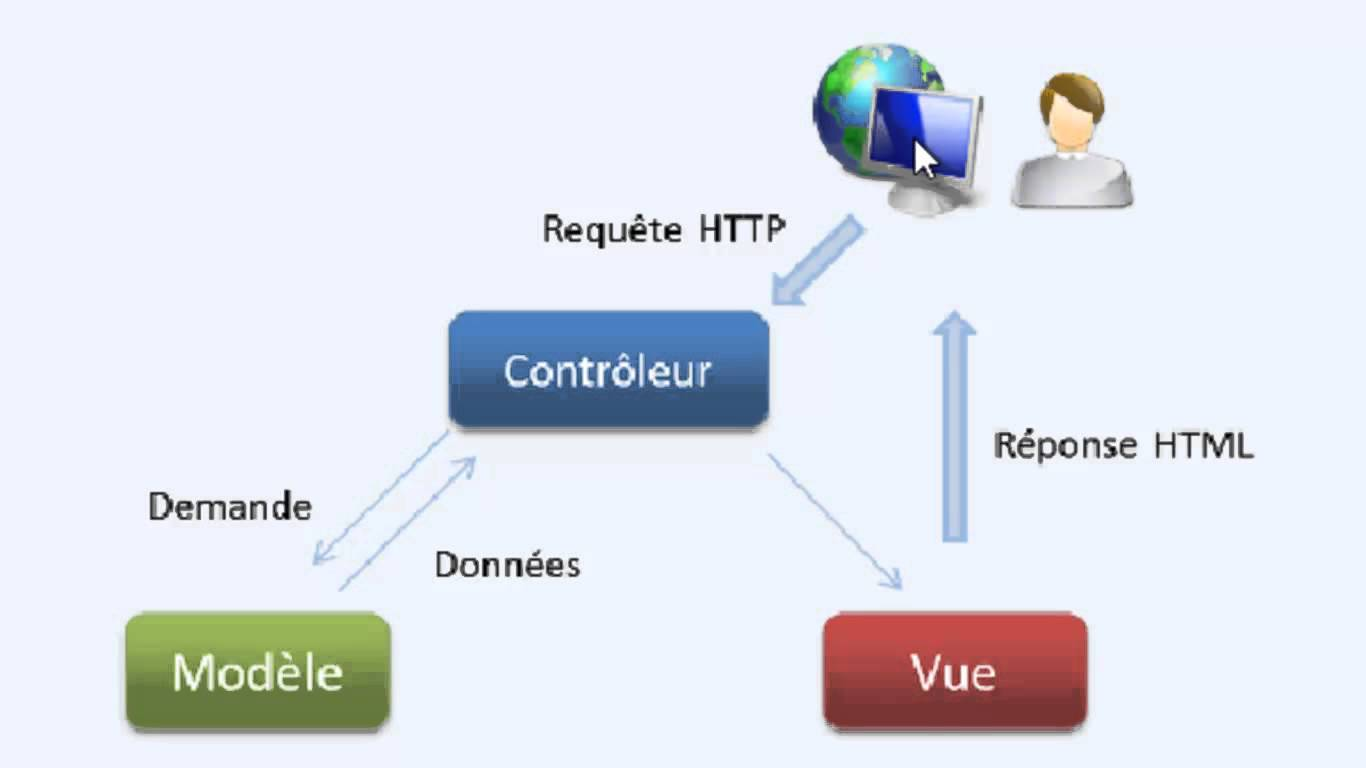
\includegraphics[width=10cm]{images/mvc.png}
     \caption{Architecture MVC}
     \label{fig:my_label}
 \end{figure}